\section{GRT} %TODO GTR Kapitel
\subsection{Eintragen einer Funktion}
\begin{paracol}{2}
\begin{flushleft}
Mit dem Grafiktaschenrechner kann man sich die Graphen verschiedener Funktionen anzeigen lasse. Dazu geht man zuerst auf und trägt dort unter  y1, y2,y3, die gewünschten Funktionen ein. Funktionen, die gezeichnet werden sollen, müssen ausgewählt werden, indem auf das Gleichheitszeichen gedrückt wird und dieses schwarz hinterlegt bleibt. 

\end{flushleft}	
\switchcolumn
\begin{flushright}
\includegraphics[width=6cm]{Media/GRT/Visualisierung/einsetzen_eines_wertes_in_Funktion/einsetzen_eines_wertes_in_Funktion}
\end{flushright}
\end{paracol}

\subsection{Anpassen des Fensterbereiches des Graphen}
\begin{paracol}{2}
\begin{flushleft}
Um das Window anzupassen, in dem der Graphen darsgestellt wird, muss man zuerst \gtr{2nd} und \gtr{window} drücken. Anschließend unterscheidet man zwischen den Werten. 
	\begin{itemize}
		\item[] \texttt{Xmin} Dieser Wert bezeichnet den mindest Wert auf der X-Achs, der zu sehen sein wird
		\item[] \texttt{Xmax} Dieser Wert bezeichnet den maximalen Wert, der auf der X-Achse zu sehen sein wird.
	\end{itemize}

\end{flushleft}	
\switchcolumn
\begin{flushright}
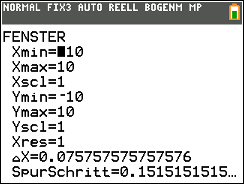
\includegraphics[width=6cm]{Media/GRT/Visualisierung/Fensterbereich_anpassen/fenster}
\end{flushright}
\end{paracol}

\begin{itemize}
	\item[] \texttt{Xscl} Dieser Wert bezeichnet die Schrittlänge auf der X-Achse 
	\item[] \texttt{Ymin} Dieser Wert bezeichnet den minimal zu sehenden Y-Wert auf der Y-Achse
	\item[] \texttt{Ymax} Dieser Wert bezeichnet den maximalen zu sehenden Y-Wert auf der Y-Achse
	\item[] \texttt{Yscl} Dieser Wert bezeichnet die Schrittlänge auf der Y-Achse
\end{itemize} Beim dem Angeben der Werte ist darauf zu achten, dass jegliche negativen Werte nicht mit dem Rechenminus, sonder mit dem Vorzeichenminus angegeben werden. Wurde der Window Bereich eingestellt, kann man im Anschluss mit der Taste \gtr{graph} zu der Ansicht des Koordinatensystems wechseln.
Ist der Graph nicht zu sehen, kann man auch über \gtr{zoom} und anschließend \texttt{zoomStandart} sich wieder die ursprüngliche Einstellung herstellen. 

\subsection{Komplett Reset}
\begin{paracol}{2}
\begin{flushleft}
	Sollte der Fall eines Fehlers auftreten, so ist das maximalinvasivste ein Reset des Taschenrechners, welcher durch die Tagenfolge \gtr{2nd} und \gtr{+}. Anschließend wählt man \texttt{reset} aus.
\end{flushleft}
\switchcolumn
\begin{flushright}
	\includegraphics[width=6cm]{Media/GRT/Visualisierung/komplett_reset/komplett_reset}
\end{flushright}	
\end{paracol}

\subsection{Einsetzen von Werten in eine Funktion}
\begin{paracol}{2}
\begin{flushleft}
	Mit den Tasten \gtr{2nd} und \gtr{trace} lässt sich das Menü zum Berechnen von verschiedenen Funktionsberechnungen aufrufen. Wählt man nun hier \texttt{1} , so kann man einen Wert in eine Funktion einsetzten für die Variable $x$.\\
	Die Dokumentation erfolgt hierbei wie folgt: \\
	\[{value(y_1,Wert)\rightarrow y=Wert}\]
	
\end{flushleft}
\switchcolumn
\begin{flushright}
	\includegraphics[width=6cm]{Media/GRT/Visualisierung/einsetzen_eines_wertes_in_Funktion/einsetzen_eines_wertes_in_Funktion}
\end{flushright}
\end{paracol}
\pagebreak
\subsection{Schnittpunkt ermitteln}

\begin{paracol}{2}
\begin{flushleft}
	Mit den Tasten \gtr{2nd} und \gtr{trace} lässt sich das Menü zum berechnen von verschiedenen Funktionsberechnungen aufrufen. Wählt man\texttt{5}, so kann man den Schnittpunkt von zwei Funktionen berechnen lassen. Hierfür muss man im ersten Schritt die erste Funktion auswähle und anschließend die zweiten und den ungefähren Schnittpunkt der beiden Funktionen.
	\[intersect(y_1,y_2)\rightarrow \quad x=\quad y=\]
	
\end{flushleft}
\switchcolumn
\begin{flushright}
	\includegraphics[width=6cm]{Media/GRT/Visualisierung/Schnittpunkt_ermitteln/Schnittpunkt_ermitteln_1}
	\includegraphics[width=6cm]{Media/GRT/Visualisierung/Schnittpunkt_ermitteln/Schnittpunkt_ermitteln_2}
	\includegraphics[width=6cm]{Media/GRT/Visualisierung/Schnittpunkt_ermitteln/Schnittpunkt_ermitteln_3}
	\includegraphics[width=6cm]{Media/GRT/Visualisierung/Schnittpunkt_ermitteln/Schnittpunkt_ermitteln_4}
\end{flushright}
\end{paracol}

\subsection{Lösen von Gleichungen}
Ist eine Gleichung mit einer Unbekannten in der Grundform $=0$ gegeben, so kann man diese leicht mit dem GTR lösen.

\begin{paracol}{2}
	\begin{flushleft}
	Zuerst erfolgt das Eintragen der Funktion in dem, indem die Funktionen eingetragen werden. Dieses wird aufgerufen, indem man die Taste \gtr{y=} drückt.
		Anschließend drückt man die Taste \gtr{graph}, um sich den Graphen anzeigen zu lassen. 
	\end{flushleft}
\switchcolumn
	\begin{flushright}
	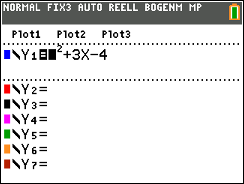
\includegraphics[width= 6cm]{Media/GRT/Visualisierung/loesen_gleichung/loesen_gleichung_1 .png}
		\end{flushright}
\end{paracol}


\begin{paracol}{2}
	\begin{flushleft}
	Um nun die Gleichung nach Null aufzulösen, wählt man \gtr{2nd} und \gtr{trace} und wählt Null aus.
		\end{flushleft}
\switchcolumn
	\begin{flushright}
	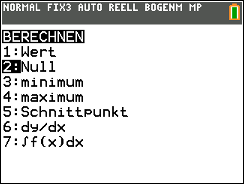
\includegraphics[width= 6cm]{Media/GRT/Visualisierung/loesen_gleichung/loesen_gleichung_2.png}
		\end{flushright}
\end{paracol}

\begin{paracol}{2}
	\begin{flushleft}
	Anschließend müssen die Grenzen bestimmt werden, indem der Taschenrechner die Nullstellen bestimmen soll. Das Wählen der ersten Grenze sollte überhalb der ersten Nullstelle geschehen.
		\end{flushleft}
\switchcolumn
	\begin{flushright}
	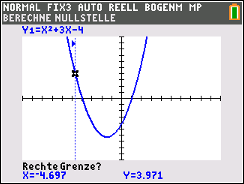
\includegraphics[width= 6cm]{Media/GRT/Visualisierung/loesen_gleichung/loesen_gleichung_3.png}
		\end{flushright}
\end{paracol}

\begin{paracol}{2}
	\begin{flushleft}
	Das Wählen der rechten Grenze geschieht unterhalb der Nullstelle.
		\end{flushleft}
\switchcolumn
	\begin{flushright}
	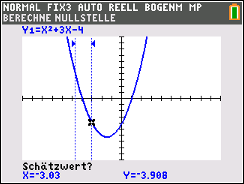
\includegraphics[width= 6cm]{Media/GRT/Visualisierung/loesen_gleichung/loesen_gleichung_4.png}
		\end{flushright}
\end{paracol}

\begin{paracol}{2}
	\begin{flushleft}
	Um schlussendlich
		\end{flushleft}
\switchcolumn
	\begin{flushright}
	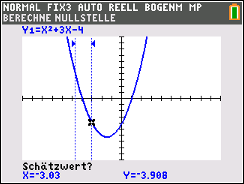
\includegraphics[width= 6cm]{Media/GRT/Visualisierung/loesen_gleichung/loesen_gleichung_4.png}
		\end{flushright}
\end{paracol}

\pagebreak

\pagebreak
